\documentclass{fefu_thesis/cls/fefu}

\usepackage{float}
\usepackage{caption}
\usepackage{subcaption}
\usepackage{hyperref}
\usepackage{algorithm}
\usepackage{algpseudocode}
\usepackage{amsmath}

\newenvironment{algo}[1][]
  {\begin{algorithm}[#1]
     \selectlanguage{english}
     \floatname{algorithm}{Алгоритм}
  }
  {\end{algorithm}}

\algdef{SE}[DOWHILE]{Do}{DoWhile}{\algorithmicdo}[1]{\algorithmicwhile\ #1}%

\newcommand*\gsegment[1]{\overline{#1}}
\newcommand*\gline[1]{\overleftrightarrow{#1}}
\newcommand*\talgref[1]{Алгоритм \ref{#1}}

\author{Терехов Дмитрий Евгеньевич}
\title{Полигонизация текстур и упаковка полигональных текстур в атлас}
\setfaculty{09.04.01 Информатика и вычислительная техника}
\setprogram{Искусственный интеллект и большие данные}
\setgroup{М9119-09.04.01иибд}
\setsupervisor{Сапрыкина Елена Валерьевна}{}
\setdirector{Мирин Илья Геннадьевич}{}
\setsecretary{Сапрыкина Елена Валерьевна}{}

\addbibresource{references.bib}

\begin{document}
    \maketitle{practice}
    \begin{abstract}
        В данной работе представлены два эффективных алгоритма: генерация текстурного меша с последующим упрощением и упаковка полигональных текстур в атлас. Оба алгоритма работают с полигонами следующих типов: невыпуклые, полигоны с дырами, полигоны, состоящие из нескольких контуров.

        \textit{Ключевые слова: генерация меша, упрощение полигонов, упаковка в контейнеры.}
    \end{abstract}
    \pagebreak
    \tableofcontents
    \pagebreak
    {\centering\section*{Введение}}
    Целью работы является решение задач упрощения полигонов и упаковки, которые играют важную роль в таких прикладных областях, как компьютерная графика, GIS системы, промышленность и т.д. Решение этой задачи также опирается на прикладную область: компьютерную графику, а именно автоматическую генерацию текстурного меша с последующей упаковкой полигональных текстур в текстурные атласы.

    Упаковка в текстурные атласы это один из этапов подготовки ассетов-текстур для оптимального использования: маленькие текстуры становятся частью большого изображения -- текстурного атласа. Это позволяет минимизировать затраты по памяти, а также уменьшить количество вызовов на отрисовку. Полигонизация текстур позволяет уменьшить количество вызовов фрагментного шейдера, путем минимизации площади пустых пикселей, входящих в меш. Также это позволяет упаковать больше текстур в атлас, т.к. в полигональном виде они занимают меньшую площадь.

    К сожалению, нет открытых программных пакетов или статей, которые решают поставленные задачи. Все программные пакеты являются проприетарными, а известные статьи решают данные задачи в очень упрощенном виде. Это и послужило мотивацией для проведение исследований и создания новых алгоритмов.

    В разделе "Раз" более подробно описывается проблема, подлежащая решению, дается обзор теоретических положений и практических подходов к решению поставленных задач.

    В разделе "Два" предлагается теоретическое решение, формируются критерии оценки эффективности алгоритмов, обоснование их корректности. Также приводится описание вспомогательных и основных алгоритмов.

    В разделе "Три" описывается применение результатов исследования в реальном проекте -- игровом движке с открытым исходным кодом <<Citrus>>.

    \section*{Глоссарий}
    \section{Задачи упрощения полигонов и упаковки в контейнеры}

    Целью работы является решение задач упрощения полигонов и упаковки, которые играют важную роль в таких прикладных областях, как компьютерная графика, GIS системы, промышленность и т.д. Решение этой задачи также опирается на прикладную область: компьютерную графику, а именно автоматическую генерацию текстурного меша с последующей упаковкой полигональных текстур в текстурные атласы.

    \subsection{Генерация текстурного меша}

    Полигональный меш (полигональная сетка) -- это совокупность вершин, рёбер и граней, которые определяют форму многогранного объекта в трёхмерной компьютерной графике и объёмном моделировании. В двумерной компьютерной графике меши используются для вершинной и скелетной анимации.

    \begin{figure}[H]
        \centering
        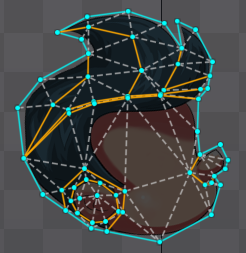
\includegraphics[scale=0.5]{images/spine_mesh.png}
        \caption{2D меш}
    \end{figure}

    Для того, чтобы отрисовать изображение на экране, необходимо пройти через графический конвейер. Обязательными и важнейшими этапами графического конвейера являются исполнение вершинного и фрагментного шейдеров, которые запускаются для каждой вершины и каждого фрагмента (пикселя) соответственно. После вызова фрагментного шейдера полученный цвет фрагмента смешивается с цветом фрагмента в буфере кадра. Многие изображения содержат огромное количество прозрачных пикселей. Вызов фрагментного шейдера для таких пикселей часто является бессмысленным, так как прозрачных пиксель при смешивании никак не повлияет на цвет на экране.
    Эти размышления приводят к одному из способов оптимизации: создание полигонального меша для изображения таким образом, чтобы минимизировать число вершин и пустых пикселей, занимаемых площадью меша.
    %МБ ВСТАВИТЬ КАРТИНКУ ГРАФИЧЕСКОГО ПАЙПЛАЙНА%

    \begin{figure}[H]
        \centering
        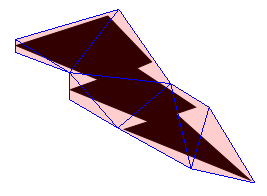
\includegraphics{images/Thunder_approx.png}
        \caption{Полигональный меш с 10 вершинами}
    \end{figure}

    Для GIS систем разработали множество алгоритмов упрощения кривой: алгоритм Ramer–Douglas–Peucker\cite{Ramer}\cite{DouglasPeucker}, алгоритм радиального расстояния\cite{PolylineSimplification}, алгоритм Visvalingam–Whyatt\cite{VisvalingamWhyatt}, упрощение Opheim\cite{Opheim} и Lang\cite{Lang}, алгоритм Zhao–Saalfeld\cite{ZhaoSaalfeld}, алгоритм Reumann-Witkam\cite{ReumannWitkam}.

    Однако в данной работе задача упрощения полигонов применяется в контексте текстурного меша. Ключевыми отличиями данной прикладной задачи от общей является минимизация не только количества вершин, но и площади прозрачных пикселей (или добавочной площади), а также ограничение, которое не позволяет нарушать границы исходных полигонов (контур изображения). Описанные выше алгоритмы можно адаптировать, чтобы они соответствовали ограничению. К сожалению, данные алгоритмы совсем не рассчитаны на минимизацию добавочной площади, а также часто приходят в тупиковую ситуацию, когда все ещё требует уменьшить количество вершин, но возможных трансформаций не существует. Решение данных проблем привело к созданию алгоритма упрощения множества простых полигонов с дырками.

    \subsection{Упаковка текстур в атласы}

    Упаковка в текстурные атласы это один из этапов подготовки ассетов-текстур для оптимального использования: маленькие текстуры становятся частью большого изображения -- текстурного атласа. Под­текстуры отображаются на объект, используя UV ­преобразование, при этом координаты в атласе задают, какую часть изображения нужно использовать. В приложениях нередко используется множество маленьких текстур, причём переключение с одной текстуры на другую является относительно медленным процессом. Поэтому в подобных ситуациях целесообразно применение одного большого изображения вместо множества маленьких. Также текстурные атласы помогают сэкономить память при помощи полигональной упаковки и\textbackslash или алгоритмов сжатия.

    Задача упаковки в контейнеры -- NP-трудная комбинаторная задача. Задача заключается в упаковке объектов предопределённой формы в конечное число контейнеров предопределённой формы таким способом, чтобы число использованных контейнеров было наименьшим или количество или объём объектов (которые упаковывают) были наибольшими. В данной работе предлагается решение 2D irregular bin packing problem, т.е. упаковка полигональных объектов в прямоугольные контейнеры.

    Для упаковки прямоугольных объектов существует множество эвристических алгоритмов\cite{ThousandWayToPackBin}, которые хорошо показывают себя на практике. В области упаковки полигонов существуют различные подходы.

    No-fit polygon\cite{NofitPolygon}\cite{NofitPolygon2} -- это конструкция, которая определяет все положения, которые могут принимать 2 произвольных многоугольника относительно друг друга так, чтобы они соприкасались, но не перекрывались. Часто методы на основе no-fit polygon используют для решения задачи раскроя на производстве, где форма вырезаемых объектов несложная и заранее известна.

    Swarm intelligence (роевой интеллект) -- метод оптимизации, который описывает коллективное поведение децентрализованной самоорганизующейся системы: колонии светлячков\cite{FireFly}, муравьев\cite{AntColony}, пчел\cite{PlayrixArticle}, particle swarm optimization\cite{PSO}.

    Генетический алгоритм\cite{JAKOBS1996165} -- это эвристический алгоритм поиска, используемый для решения задач оптимизации и моделирования путём случайного подбора, комбинирования и вариации искомых параметров с использованием механизмов, аналогичных естественному отбору в природе.

    К сожалению, результаты прочитанных статей не удовлетворяют нужды упаковки текстур в атласы, поэтому данная работа предлагает собственную реализацию Memetic algorithm -- расширение генетического алгоритма, которое использует локальный поиск для уменьшения вероятности преждевременной сходимости. Разработанный алгоритм способен упаковывать изображения, на которых находятся множество разрозненных объектов с дырами.

    \section{Алгоритмы, структуры данных и математические методы}
    \subsection{Пайплайн полигональной упаковки}
    \begin{itemize}
        \item Трассировка контура изображений;
        \item Аппроксимация полученных контуров;
        \item Упаковка полигональных изображений в текстурные атласы.
    \end{itemize}
    \subsection{Трассировка контура}
    Алгоритмы выделения контура можно разделить на 3 типа: обход попиксельно, обход повершинно, run-data.
    \subsubsection{Обход попиксельно}
    Метод выделения контура обходом попиксельно начинает с какого-либо стартового пикселя и пиксель за пикселем обходит контур изображения предопределенным образом, а затем сохраняет их координаты в памяти в соответствии с порядком трассировки. Наиболее известные алгоритмы обхода контура попиксельно: Moore-neighbor tracing\cite{MoorNeighbor}, radial sweep\cite{RadialSweep} и алгоритм Theo Pavlidis\cite{TheoPavlidis}.
    \subsubsection{Обход повершинно}
    Метод выделения контура обходом повершинно отличается от обхода попиксельно лишь тем, что обход осуществляется по границам пикселя.
    \subsubsection{Run-data}
    Run-data методы выделения контура проходят по изображению сканирующей линией оставляя определенные метки на встреченном граничном пикселе. Далее по расставленным меткам восстанавливается контур изображения. Примеры методов этой группы: run-type direction code\cite{Miyatake1997}, методы, основанные на PXY таблице\cite{Shoji}. Отличительной особенностью run-data методов является возможность выделения внешних и внутренних контуров, сохраняя иерархию. Так же способ обхода изображения в некоторых алгоритмах позволяет не держать в памяти изображение целиком.

    Было решено выбрать алгоритм именно из этой группы методов, так как необходимо выделять дырки на объектах. За основу был взят алгоритм Suzuki Satoshi \cite{SuzukiAlgorithm}, использующийся в библиотеке OpenCV. Алгоритм способен построить иерархию контуров и типизировать их на границы и дыры.

    \begin{figure}[H]
        \centering
        \begin{subfigure}[t]{.49\linewidth}
            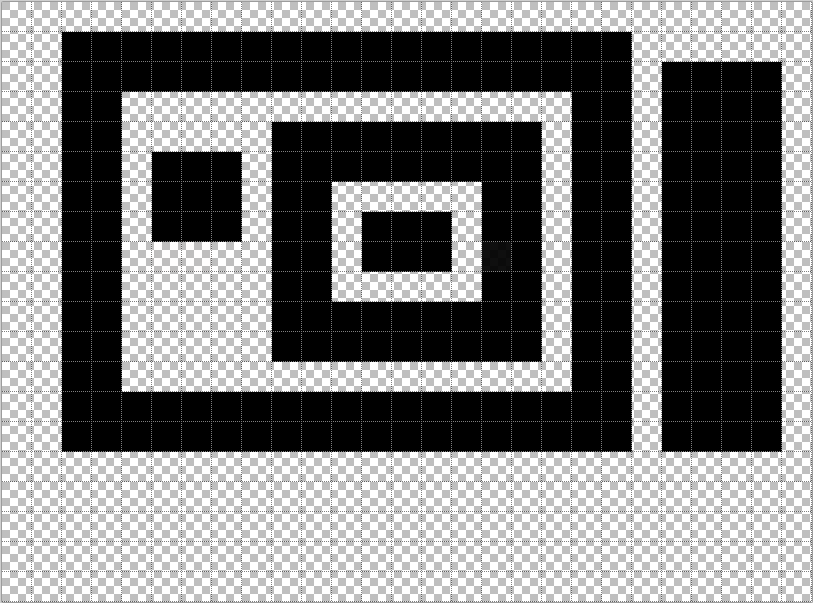
\includegraphics[scale=0.4]{images/SuzukiExample_upscaled.png}
            \caption{Изображение}
        \end{subfigure}
        \begin{subfigure}[t]{.49\linewidth}
            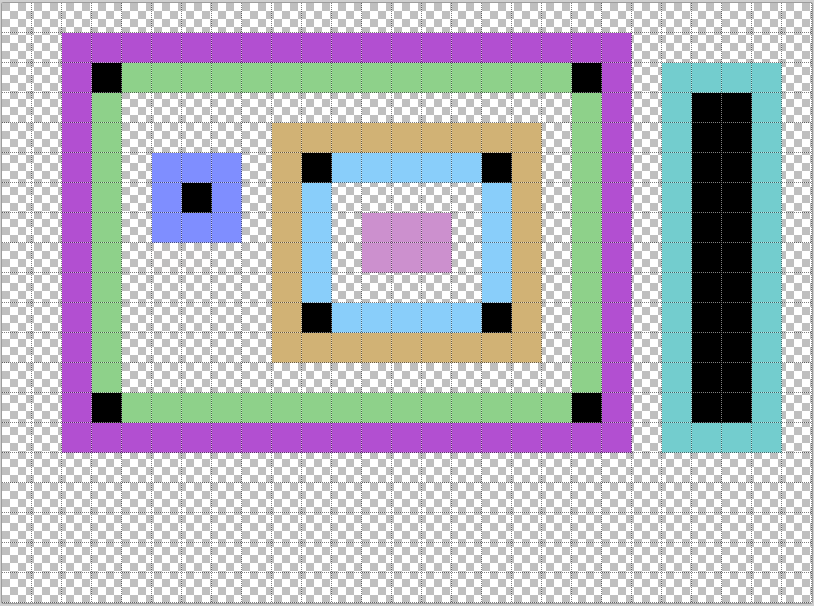
\includegraphics[scale=0.4]{images/SuzukiExample_contours_upscaled.png}
            \caption{Контуры изображения}
        \end{subfigure}
        \begin{subfigure}[t]{.99\linewidth}
            \centering
            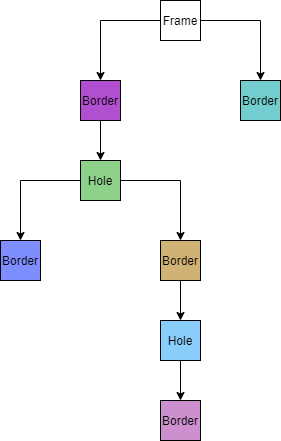
\includegraphics[scale=0.7]{images/SuzukiExample_hierarchy.png}
            \caption{Иерархия контуров}
        \end{subfigure}
        \caption{Пример работы алгоритма Suzuki Satoshi}
    \end{figure}

    Алгоритм оперирует с дискретными координатами пикселей, а в компьютерной графике UV координаты это непрерывные вещественные числа. Такое представление контура создает некоторые проблемы.

    Во-первых, может получится контур с самопересечениями, которые нетривиально разрешить. На \ref{SelfIntersectingContours} изображены примеры контуров с самопересечением. Красным обозначены вершины, которые алгоритм посещает дважды.
    \begin{figure}[H]
        \centering
        \begin{subfigure}[t]{.49\linewidth}
            \centering
            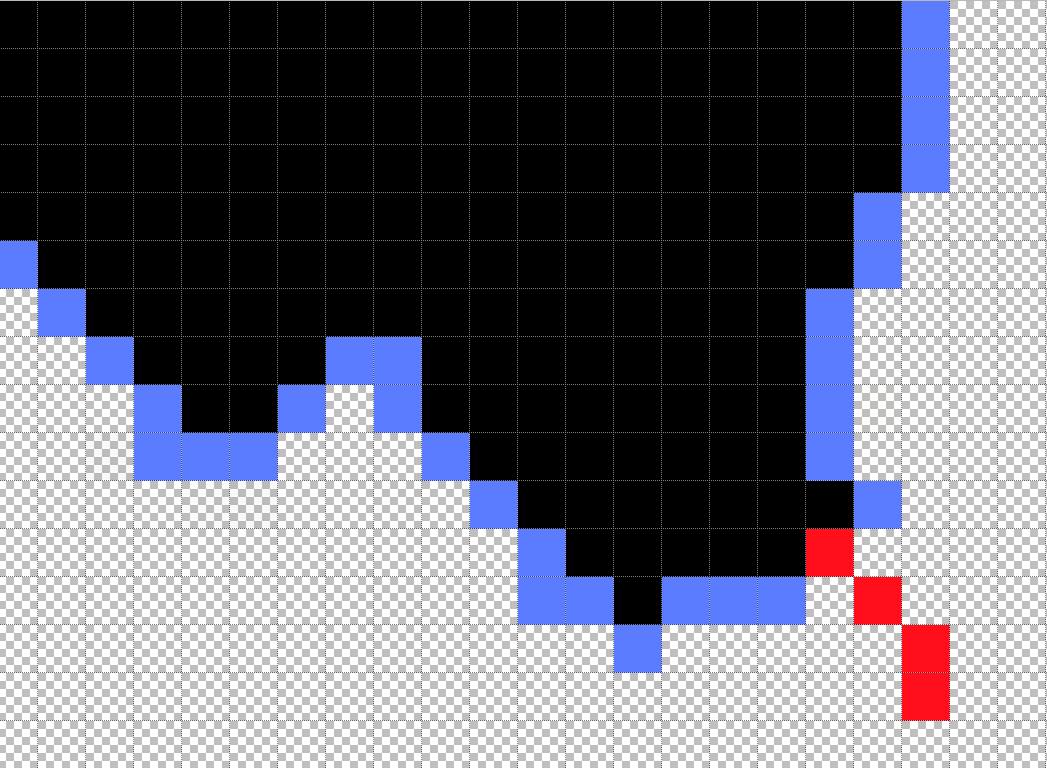
\includegraphics[scale=0.2]{images/SelfIntersectingContour1.png}
            \caption{Изображение}
        \end{subfigure}
        \begin{subfigure}[t]{.49\linewidth}
            \centering
            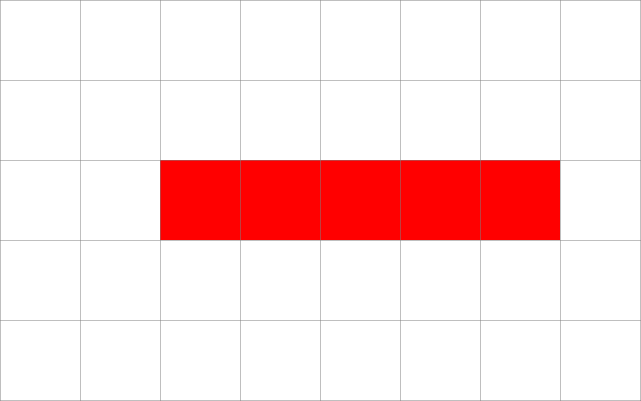
\includegraphics[scale=0.4]{images/SelfIntersectingContour2.png}
            \caption{Контуры изображения}
        \end{subfigure}
        \caption{Примеры контуров с самопересечением}
        \label{SelfIntersectingContours}
    \end{figure}

    Во-вторых, некоторые пиксели при отрисовке будут обрезаны, т.к. дискретные координаты пикселя в прямой интерпретации в качестве UV координат будут являются координатами левого верхнего угла пикселя. В таком случае, нижние и правые пиксели просто не будут учтены при отрисовке.

    \begin{figure}[H]
        \centering
        \begin{subfigure}[t]{.33\linewidth}
            \centering
            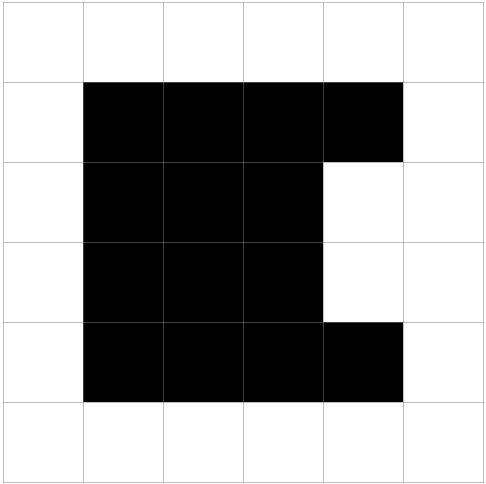
\includegraphics[scale=0.2]{images/SuzukiExample2.png}
            \caption{Изображение}
        \end{subfigure}
        \begin{subfigure}[t]{.33\linewidth}
            \centering
            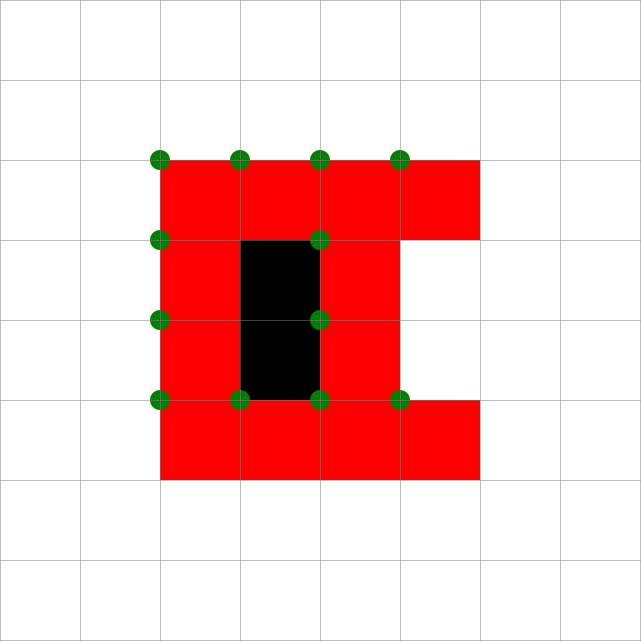
\includegraphics[scale=0.2]{images/SuzukiExample2_uvs.png}
            \caption{Контуры изображения + UV координаты}
        \end{subfigure}
        \begin{subfigure}[t]{.32\linewidth}
            \centering
            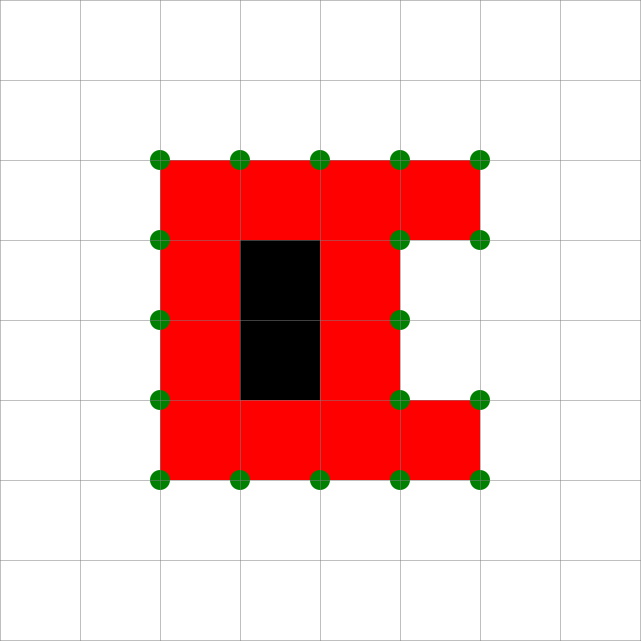
\includegraphics[scale=0.2]{images/SuzukiExample2_wanted_uvs.png}
            \caption{Контур изображения и желаемые UV координаты}
        \end{subfigure}
        \caption{Проблема неправильных UV координат}
    \end{figure}

    Для решения данных проблем был разработан алгоритм, который превращает попиксельный контур в повершинный.
    \begin{algo}[H]
        \setstretch{1}
        \caption{Pixel contour to vertex contour}
        \begin{algorithmic}[1]
            \Procedure{ToVertexContour}{$contour, type$}
                \State $vertices$ $=$ $[]$
                \State $prevTexel$ $=$ $contour$$[0]$
                \If{$type == Hole$}
                    \State $verticies.Add(position)$
                \EndIf
                \State $position$ $=$ $type$ $==$ $Outer$ $?$
                \State $prevTexel$ $:$
                \State $NextCWVertex(prevTexel, NextCWVertex(prevTexel, prevTexel))$
                \For{$i = 1$ \textbf{to} $contour.Size$}
                    \State $currentTexel = contour[i]$
                    \State $position = TracePixel(prevTexel, currentTexel, position, vertices)$
                    \State $prevTexel = currentTexel$
                \EndFor
                \State $TracePixel(prevTexel, contour[0], position, vertices)$
                \State \textbf{return} $vertices$
            \EndProcedure
            \Procedure{TracePixel}{$prevTexel, texel, position, vertices$}
                \Do
                    \State $position = NextCWVertex(prevTexel, position)$
                    \State $vertices.Add(position)$
                \DoWhile { $!IsVertexOf(texel, position)$ }
                \State \textbf{return} $position$
            \EndProcedure
        \end{algorithmic}
    \end{algo}

    Функции NextCCWVertex(texel, vertex) и NextCWVertex(texel, vertex) возвращают следующую вершину текселя против и по часовой соответственно. IsVertexOf(texel, vertex) возвращает true, если вершина принадлежит текселю.

    Для того, чтобы снизить количество вершин перед следующим этапом обработки изображения, контуры подвергаются первичной аппроксимации. Самым очевидным способом аппроксимации контура является удаление вершин лежащих на одной прямой. Также существуют алгоритмы упрощения цифровых кривых. В данной работе был реализован алгоритм Teh-Chin\cite{TehChin} c $L1$ и $k\cos$ метриками.

    \subsection{Аппроксимация полигонов}
    \label{PolygonApproximation}
    Аппроксимация полигонов для текстурных мешей отличается от аппроксимации полигонов, например, в GIS системах: запрещено нарушать искомые границы, а так же необходимо минимизировать не только количество вершин, но и добавочную площадь. Мета-алгоритм можно описать следующим образом:

    \begin{algo}[H]
        \setstretch{1}
        \caption{Meta-algorithm for a set of polygons approximation}
        \begin{algorithmic}[1]
            \Procedure{ApproximatePolygons}{$polygons, hierarchy, frameRect$}
                \State $minExtractor, topology, frame = $
                \State $Initialize(polygons, hierarchy, frameRect)$
                \While {Termination Condition is not achieved}
                    \If {$!TryApproximate(\cdots)$ and $!TryMerge(\cdots)$}
                    \State \textbf{break}
                    \EndIf
                \EndWhile
                \State \textbf{return} $RetrieveImage(\cdots)$
            \EndProcedure
        \end{algorithmic}
    \end{algo}

    На стадии инициализации создаются две модели множества полигонов. Первая модель это дерево полигонов, где каждый узел дерева это полигон $P_i$, представленный двусвязным зацикленным списком вершин $P_i = \left(v_j\right)_{j=0}^{n - 1}$, $v_{j \pm m}$ подразумевает $v_{j \pm m \pmod n}$. Корнем дерева является ограничивающая рамка ($frame$). Вторая модель ($topology$) это триангуляция Делоне с ограничениями. В реализации алгоритма использовался пакет, разработанный в рамках бакалаврской выпускной квалификационной работы \cite{Delaunay}. Триангуляция Делоне это мощнейший инструмент для проверки преобразований над полигонами, а также вычисления полигона видимости. Также на стадии инициализации происходит подсчет минимальной возможной трансформации для каждой вершины. "Стоимость" трансформации измеряется в добавочной площади. Для быстрого поиска минимальной трансформации (т.е. трансформации с минимальной стоимостью) используется сбалансированное дерево поиска ($minExtractor$).

    Далее выполняются преобразования или мерджатся полигоны, пока не условие выхода не будет достигнуто. Процедура $RetrieveImage$ возвращает объект типа $Image$. $Image$ содержит в себе все вершины и индексных массив (массив троек индексов вершин), а также массив объектов типа $ImageObject$. Объектом картинки называется граничный контур со всеми принадлежащими ему дырами. $ImageObject$ содержит в себе индексы вершин для контура и всех дыр, а также индексы троек индексов, ему принадлежащих. Данные структуры данных в дальнейшем используются для упаковки.

    \subsubsection{Преобразования над вершинами}
    Стоимостью преобразования является добавляемая площадь площадь, которая представляет из себя один или два треугольника. Возможность преобразования проверяется путем вставки в триангуляцию структурных ребер и проверки на существование определенного треугольника. Данная проверка необходима для того, чтобы избежать случаев, когда какая-то другая граница попадает в добавочную площадь.

    \begin{figure}[H]
        \centering
        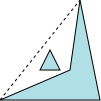
\includegraphics[scale=1]{images/triangle_existance_check.png}
        \caption{Соседняя граница попадает в добавочную площадь}
    \end{figure}

    \paragraph{Удаление вершин, лежащий на одной прямой}
    Очевидно, данная трансформация имеет нулевую стоимость и проста в реализации.
    \paragraph{Удаление вогнутого/выпуклого угла}
    Если вершина $v_i$ принадлежит границе или дыре и образует вогнутый или выпуклый угол соответственно, то возможно провести отрезок $\gsegment{v_{i - 1}v_{i + 1}}$ и удалить вершину $v_i$. Также из теоремы о двух ушах следует, что любой последовательностью  таких преобразований можно сократить дыру до треугольника. Теорема о двух ушах гласит, что в каждом просто полигоне с более чем 3 вершинами есть хотя бы 2 уха. Ухом называется вершина, соседние вершины которой можно соединить отрезком, который будет полностью лежать внутри полигона.

    \begin{figure}[H]
        \centering
        
\includegraphics[scale=1]{images/earcut.png}
        \caption{Удаление вогнутого угла}
    \end{figure}
    \paragraph{Пересечение сторон}
    Если $v_i$ образует выпуклый угол, то может существовать возможность заменить вершину $v_i$ и $v_{i + 1}$ пересечением прямых $\gline{v_{i - 1}v_i}$ и $\gline{v_{i + 1}v_{i + 2}}$. Для проверки возможности такого преобразования необходимо предварительно проверить знак параметра при пересечении прямых, используя векторное параметрическое уравнение ($\vec{r} = \vec{r_0} + t \cdot \vec{u}$).

    \begin{figure}[H]
        \centering
        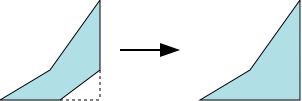
\includegraphics[scale=1]{images/bendneighbor2.png}
        \caption{Пересечение сторон}
    \end{figure}

    \paragraph{Выгибание соседней вершины}
    Данное преобразование является оптимизированной версией удаления вогнутого угла. Если линия, образованная предыдущей и пред предыдущей вершинами, пересекает сторону, образованную текущей и следующей вершинами, то существует возможность заменить предыдущую и текущую вершины пересечением линии и стороны. Аналогично для четверки следующая, последующая, текущая и предыдущая вершин.

    Данное преобразование является оптимизированной версией удаления вогнутого угла. Если $\gline{v_{i - 2}v_{i - 1}}$ пересекает $\gsegment{v_iv_{i + 1}}$, то можно не отрезать весь угол, а заменить $v_{i - 1}$ и $v_{i}$ пересечением. Аналогично работает для $\gline{v_{i + 2}v_{i + 1}}$ и $\gsegment{v_iv_{i - 1}}$.

    \begin{figure}[H]
        \centering
        
\includegraphics[scale=1]{images/bendneighbor.png}
        \caption{Выгибание соседней вершины}
    \end{figure}

    \paragraph{Выгибание двух соседних вершин}
    Пусть $v_{i - 1}$, $v_{i}$ и $v_{i + 1}$ являются вершинами выпуклых углов, тогда можно попробовать заменить все 3 вершины пересечением $\gline{v_{i - 2}v_{i - 1}}$ и $\gline{v_{i + 2}v_{i + 1}}$ с вертикальной или горизонтальной прямой, проходящей через $v_i$.
    \begin{figure}[H]
        \centering
        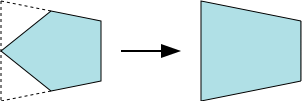
\includegraphics[scale=1]{images/bendoutboth.png}
        \caption{Выгибание двух соседних вершин к вертикальной прямой}
    \end{figure}
    \paragraph{Удаление треугольной дыры}
    Если дыра упростилась до треугольника и внутри нет граничных полигонов, то единственная возможная трансформация для этих вершин -- удаление всей треугольной дыры. Это также влечет за собой удаление полигона из дерева полигонов.

    \begin{figure}[H]
        \centering
        
\includegraphics[scale=1]{images/remove_triangular_hole.png}
        \caption{Удаление треугольной дыры}
    \end{figure}

    \subsubsection{Мердж полигонов}
    В каждой полигональной дыре (включая $frame$) выбирается 2 пары последовательных вершин из разных полигонов, которые образуют минимальный четырехугольник, который не пересекает другие стороны. Данные 4 вершины являются точками мерджа.
    \begin{figure}[H]
        \centering
        \begin{subfigure}[t]{\linewidth}
            \centering
            
\includegraphics[scale=1]{images/polygonmerge.png}
            \caption{Мердж границы с дырой}
        \end{subfigure}
        \begin{subfigure}[t]{\linewidth}
            \centering
            
\includegraphics[scale=1]{images/polygonmerge2.png}
            \caption{Мердж границы с границей}
        \end{subfigure}
    \end{figure}

    \subsubsection{Применение преобразований}
    На каждой итерации цикла применяется аппроксимирующее преобразование с минимальной стоимостью. После применения преобразования пересчитываются преобразования соседних вершин.
    Аппроксимация соседних контуров или объемлющей дыры могут повлияет на валидность посчитанного преобразования, поэтому при неудачной попытке преобразование для вершины пересчитывается и вершина кладется обратно в $minExtractor$. Такой ленивый пересчет позволяет избежать огромных временных затрат, так как любая трансформация может в худшем случае повлиять на трансформацию $O\left(n\right)$ вершин. Однако на практике такое встречается редко.

    \subsubsection{Вычислительная устойчивость}
    Вычислительная устойчивость алгоритма достигается использованием вычислительно устойчивых геометрических предикатов, разработанных Jonathan Shewchuk\cite{shewchuk97a}. Данные предикаты также используются для построения Делоне с ограничениями.
    \subsubsection{Меш}
    В дальнейшем для упаковки и отрисовки в атлас понадобится меш всех объектов на изображении. Так как для аппроксимации создается триангуляция Делоне, то достаточно выбрать из неё нужные треугольники. Для этого достаточно запустить обход в глубину триангуляции. Основой триангуляции является структура данных Halfedge \cite{Halfedge}, представляющая собой ориентированное ребро с указателем на следующее и соседнее (ориентированное в обратном направлении) ребро. Каждое структурное (constrained) ребро триангуляции является ребром одного из полигонов. Значит, при переходе через такое ребро мы входим или выходим в/из площади объекта на картинке.

    \begin{algo}[H]
        \setstretch{1}
        \caption{Retrieve image mesh}
        \begin{algorithmic}[1]
            \State $used \gets \emptyset$
            \State $faceList \gets []$
            \State $polygonToFaceIndecies, sideToPolygon \gets Precalculate()$
            \Procedure{RetrieveMesh}{$edge, faceIndecies, faceList$}
                \If{$faceIndecies \neq null$} \Comment{Means inside a polygon}
                    \State $faceIndecies.Add(faceList.Count)$
                    \State $faceList.Add(edge.ToFace())$
                    \State $current \gets edge.Next$
                    \While{$current \neq edge$}
                        \If{$current.Twin \neq null \; \textbf{and} \; used \cap current != \emptyset$ }
                            \State $used \gets used \cup current$
                            \State $twin \gets current.Twin$
                            \State $fis \gets faceIndecies$
                            \If{$twin.IsConstrained$}
                                \State $polygon \gets sideToPolygon[edge]$ \Comment{returns polygon or null}
                                \State $fis \gets polygonToFaceIndecies[polygon]$
                            \EndIf
                            \State $RetrieveMesh(twin, fis, faceList)$
                        \EndIf
                    \EndWhile
                \EndIf
                \State $current \gets current.Next$
            \EndProcedure
        \end{algorithmic}
    \end{algo}

    \subsection{Генетический алгоритм}
    Основная идея всех эволюционных алгоритмов одинаково: популяция особей в некоторой среде конкурирует за ограниченные ресурсы, конкуренция приводит к естественному отбору -- выживает наиболее приспособленный. Каждая особь представляет собой элемент в области определения функции приспособленности (fitness or evaluation function, функции оценки), которую необходимо минимизировать. Изначально создается популяции из случайных значений из области определения функции. Затем отбираются лучшие особи, которые подвергаются воздействую операторов вариации (рекомбинации и\textbackslash или мутации). Из полученной популяции только часть наиболее приспособленных особей доживает до нового поколение. И так повторяется до тех пор, пока не будет достигнуто желаемое решение. Генетический мета-алгоритм показан в \talgref{meta-genetics}.

    \begin{algo}[H]
        \setstretch{1}
        \caption{Генетический мета-алгоритм}
        \label{meta-genetics}
        \begin{algorithmic}[1]
            \State $INITIALIZE$ population with random candidate solution
            \State $EVALUATE$ each candidate
            \While{$TERMINATION\; CONDITION$ \textbf{is not} satisfied}
                \State $SELECT$ parents
                \State $RECOMBINE$ pairs of parents
                \State $MUTATE$ offspring
                \State $EVALUATE$ new candidates
                \State $SELECT$ individuals for the next generation
            \EndWhile
        \end{algorithmic}
    \end{algo}

    Стоит отметить, что все компоненты, кроме оценки особей, являются стохастическими. Например, мутация задевает случайную часть решения, а слабые особи имеют малый шанс выиграть в естественном отборе.

    \subsubsection{Составные части генетического алгоритма}
    \paragraph{Инициализация}
    Чаще всего изначальная популяция просто заполняется случайно сгенерированными особями. Однако, могут использоваться специфические для данной проблемы эвристики, которые позволяют создать более приспособленную изначальную популяцию.
    \paragraph{Функция оценки}
    Функция оценки задает требования, к которым популяция вынуждена адаптироваться. Технически, это функция, которая определяет меру качества особи. Смысл всего генетического алгоритма в минимизации функции оценки для популяции, чтобы достичь наиболее качественного решения.
    \paragraph{Популяция}
    Популяции это набор особей. Практически во всех вариантах эволюционных алгоритмов размер популяции постоянен. Отбор берет во внимание всю популяцию целиком, а не отдельно каждого индивида.
    \paragraph{Механизм отбора родителей}
    Механизм отбора родителей используется, чтобы выбрать наиболее хороших особей для того, чтобы они стали родителями для следующего поколения. Отбор родителей необходим, чтобы повысить качество будущего поколения. Для создания потомства к родителям применяют операторы вариации. Выбор родителей всегда вероятностный. Более приспособленные особи имеет более высокий шанс стать родителями, но менее приспособленным особям дается малый шанс, иначе поиск решения будет слишком жадным.
    \paragraph{Операторы вариации. Мутация и рекомбинация}
    Роль операторов вариации -- создание новых особей из старых. Обычно, разделяют операторы вариации разделяют на 2 группы по арности: унарная и n-арная версии. Все операторы вариации, обычно, стохастические. Исключением является применение операторов вариации, в которых заложено знание о проблеме. Таким образом, можно исключить образование заведомо неверных решений в популяции либо всегда создавать решения лучше их родительских.

    Унарный оператор вариации, обычно, называют мутацией. Мутация применяется к одной особи, производя из неё новую слегка измененную особь. Роль мутации заключается в исследовании новых мест в области значений функции оценки. Мутация позволяет избежать преждевременной сходимости в локальном минимуме.

    Бинарный оператор вариации, обычно, называют рекомбинацией или кроссовером. Как следует из названия, такой оператор совмещает информацию от двух родителей, сохраняя свойства от обоих. Роль кроссовера заключается в эксплуатации области значения функции оценки, занимаемой текущим поколением популяции.
    \paragraph{Механизм отбора выживших}
    После создания новых особей необходимо выбрать, какие особи составят следующее поколение популяции. Как и механизм отбора родителей, механизм отбора выживших является стохастическим и дает шанс менее приспособленным особям быть отобранными в новое поколение.
    \paragraph{Условие выхода}
    Условие выхода очень сильно зависит от задачи. Часто используют следующие варианты или их комбинации:
    \begin{itemize}
        \item Популяция сошлась к какому-то решение;
        \item Было достигнуто достаточно качественное решение;
        \item Был достигнут лимит времени на эволюцию;
        \item Прирост качества сильно замедлился;
        \item и т.д.
    \end{itemize}

    \subsection{Упаковка в атлас}
    Для упаковки в атлас мы используем классический генетический алгоритм из \talgref{meta-genetics}, но с некоторыми модификациями, о которых будет сказано позже. Для начала перечислим конкретные имплементации всех этапов генетического алгоритма для упаковки полигональных изображений в атлас.
    \subsubsection{Репрезентация особей}
    Особь является отражает решение конкретной проблемы. В нашем случае особь состоит из 2 массивов данных. В первом массиве хранятся тройки целых чисел, отвечающие за трансформацию каждого $ImageObject$ (перемещение по осям X и Y, а также поворот). В о втором массиве хранятся флаги присутствия конкретного объекта $Image$ в атласа ($true$ -- присутствует, $false$ -- отсутствует). Размер атласа подбирается отдельно и не является частью генетического алгоритма.
    \subsubsection{Популяция}
    Размер популяции константный и задается в качестве параметра для генетического алгоритма.
    \subsubsection{Механизм отбора родителей}
    Как было сказано ранее, отбор родителей это стохастический процесс, в котором более приспособленные родители имеют более высокий шанс быть выбранными, поэтому первое, что приходит на ум, это присвоить шанс выбора пропорционально значению функции оценки, то есть $P\left(i\right) = \frac{f_i}{\sum_{j=0}^{n - 1} f_i}$. Однако такое наивное решение имеет ряд недостатков:
    \begin{itemize}
        \item Выдающиеся особи быстро захватывают популяцию, что вырождается в преждевременной сходимости, часто, не к лучшему результату;
        \item Когда значение оценочной функции особей близко друг к другу, то выбор становится равномерно случайным;
        \item При применении аффинных преобразований к функции оценки, данный способ отбора начинает вести себя совершенно по-другому.
    \end{itemize}

    Отбор по рангу\cite{RankingSelection} это другой метод, вдохновленный недостатками отбору по значению оценочной функции. Данный метод сортирует популяцию по значению оценочной функции и присваивает ранг каждой особи (лучшее решение имеет ранг $n - 1$, а худшее $0$). Вероятность отбора вычисляется на основе ранга, например, линейно или экспоненциально уменьшаясь от лучшего решения к худшему,
    \begin{align*}
        P_{linear}\left(i\right) &= \frac{2 - s}{n} + \frac{2i\left(s - 1\right)}{n\left(n - 1\right)},\\
        P_{exp}\left(i\right) &= \frac{1 - e^{-i}}{c}.
    \end{align*}
    где $s$ это константа $1 < s\leq 2$, а $c$ выбирается так, чтобы сумма вероятностей равнялась $1$. В алгоритме упаковки применяется отбор по рангу с экспоненциальной формулой.

    После присвоения вероятностей выбора каждой особи необходимо составить множество родителей. Для этого существуют такие алгоритмы, как roulette wheel или tournament selection, но в алгоритме упаковки было решено использовать \textbf{stochastic universal sampling}\cite{RankingSelection}.

    \begin{algo}[H]
        \setstretch{1}
        \caption{Stochastic Universal Sampling}
        \begin{algorithmic}[1]
            \State $a$ is cumulative probability distribution
            \State $m$ is number of parents we want to selects
            \State $current \gets 1$
            \State $i \gets 1$
            \State $r \gets$ uniformly random from $\left[0, 1 / m\right]$
            \While{$current \leq m$}
                \While{$r \leq a_i$}
                    \State $parents_i \gets popoluation_i$
                    \State $r \gets 4 + 1 / m$
                    \State $current \gets current + 1$
                \EndWhile
                \State $i \gets i + 1$
            \EndWhile
        \end{algorithmic}
    \end{algo}

    \subsection{Мутация}
    В алгоритме упаковки равновероятностно выбирается одна из двух мутаций: \textbf{Reset} и \textbf{Creep}.

    \textbf{Random Resetting} мутация изменяет значение случайного гена на значение из заранее определенного диапазона. Например, ген вращения $ImageObject$ можно повторно установить в значение в диапазоне $\left[0, 359\right]$ градусов.

    \textbf{Creep} мутация добавляет какую-то малую случайную дельту к значению гена. Например, можно добавлять к гену поворота случайный поворот в диапазоне $\left[-10, 10\right]$ градусов.

    \subsection{Кроссовер}
    В алгоритме упаковки используется простейший одноточечный кроссовер, работу которого демонстрирует следующее изображение.
    \begin{figure}[H]
        \centering
        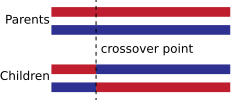
\includegraphics[scale=1]{images/OnePointCrossover.png}
        \caption{Одноточечный кроссовер}
    \end{figure}

    \subsection{Отбор выживших}
    В алгоритме используется композитная стратегия отбора выживших, состоящие из следующих стратегий отбора.

    \textbf{Age based}. Если особь прожила больше $a$ поколений, то эта особь не попадает в новое поколение.

    \textbf{Elitism}. $e$ наиболее приспособленных особей обязательно проходят в следующее поколение. Данная стратегия позволяет не потерять наиболее хорошее решение из найденных.

    \textbf{Replace worst (GENITOR)}. $m$ худших особей замещаются созданными потомками.
    \subsection{Функция оценки}
    Функция оценки включает в себя ограничения, накладываемые на решение, и задана таким образом, чтобы мотивировать популяцию эволюционировать в приемлемое решение как можно быстрее. Главными ограничениями является площадь пересечения полигонов и площадь выступов, образуемых минимальными и максимальными значениями координат.

    \begin{figure}[H]
        \centering
        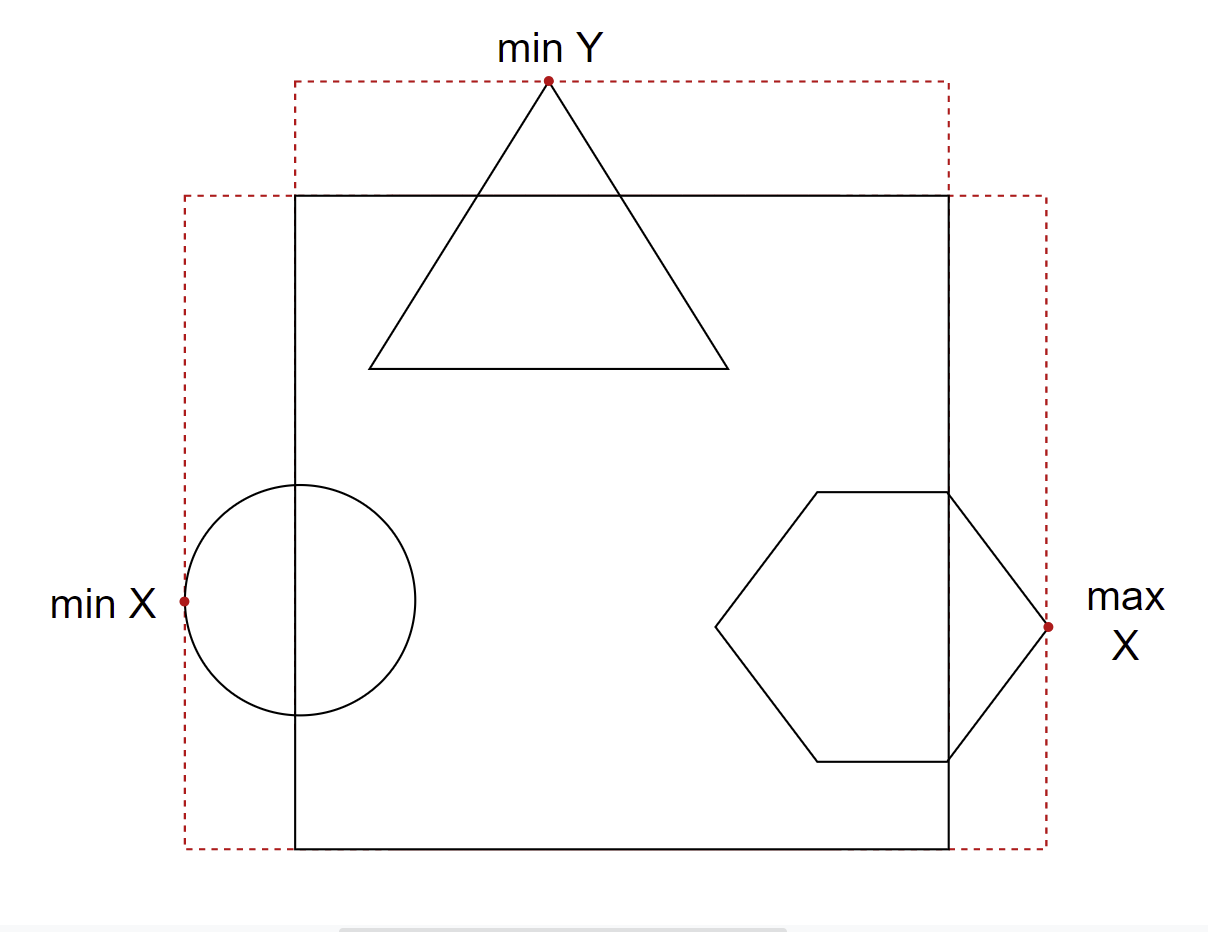
\includegraphics[scale=0.5]{images/ledges.png}
        \caption{Площадь выступов}
    \end{figure}

    Эти два ограничения мотивируют решение строиться таким образом, чтобы все фигуры попадали в атлас и не пересекались с остальными фигурами. Также в функции оценки учитывается количество изображений, не попавших в атлас, помноженное либо на среднюю площадь изображений, что мотивируют решение вобрать себя как можно больше изображений. Функция оценки это сумма перечисленных выше слагаемых с коэффициентами:
    \[
        F\left(individual\right) = a \cdot S_{intersection} + b \cdot S_{outside\;ledges} + c \cdot missing \cdot S_{avg}
    \]
    где $c$ это коэффициент, контролируемый снаружи. С его помощью можно ослабить требование к решению, что позволит алгоритму сойтись.

    Если нахождение второго и третьего слагаемых тривиально, то нахождение площади пересечения всех полигонов довольно сложно. Существуют алгоритмы, способные производить булевые операции над полигонами с дырами и самопересечениями. Например, алгоритмы Vatti\cite{Vatti}, Greiner-Hormann\cite{GreinerHormann} или Martinez\cite{Martinez}. В данной работе был реализован модифицированный алгоритм Martinez\cite{Martinez}, способный подсчитать за один проход объединение всех полигонов, однако в скорости он всё равно уступает библиотеке Clipper за авторством Angus Johnson \cite{Clipper}, которая представляет собой расширение алгоритма Vatti \cite{Vatti}. Площадь пересечения между фигурами считается, как разница площади объединения и суммы площади полигонов $S_{intersection} = S\left(\bigcup\limits_{i = 0}^{m - 1} P_i\right) - \sum\limits_{i = 0}^{m - 1}S\left(P_i\right)$.

    \subsection{Memetic algorithm}
    Данный алгоритм упаковки является расширением классического генетического алгоритма, представленного в \talgref{meta-genetics}, и является реализацией memetic algorithm, который использует процедуру локального поиска, именуемой в литературе фазой обучения (learning phase). Некоторые выбранные особи перед отбором родителей проходят проходят процедуру локального поиска, которой известна специфика решаемой проблемы и которая пытается улучшить существующее решение. В данной работе используются 2 процедуры локального поиска: \textbf{hole filling} и \textbf{physics}.

    \textbf{Hole filling}. Процедура пытается заполнить полигональные дыры объектами, которые потенциально могут поместиться в данную дыру.

    \textbf{Physics}. Используется симуляция физики при помощи известного физического движка Box2D \cite{Box2D}. Симуляция физики позволяет быстро преодолеть момент, когда между объектами остаются маленькие пересечения, от которых долго избавляется эволюция.

    \subsection{Условие выхода}
    Условия выхода имеет 2 этапа. Первый этап -- это достижение приемлемого решения. Решение считается приемлемым, если $S_{outside_ledges} = S_{intersection} = 0$. Далее дается константное количество поколений для улучшения решения.

    Условие выхода может сработать, когда ещё не все изображения упаковались (возможно, их и нельзя упаковать в тот же атлас). Для неупакованных изображений алгоритм запускается заново.

    \subsection{Выбор размера атласа}
    Размер атласа выбирается путем упаковки изображений быстрым жадным алгоритмов. Например, алгоритмом гильотины \cite{ThousandWayToPackBin}.
    \newpage
    \printbibliography
\end{document}
